\documentclass[letterpaper,12pt]{article}
\usepackage{cite}
\usepackage{graphicx}
\usepackage{amsmath}
\usepackage{adjustbox}
\usepackage{caption}
\usepackage{subcaption}
\captionsetup[figure]{labelsep=period}
\captionsetup[subfigure]{labelformat=simple} % default is 'parens'
\renewcommand\thesubfigure{\thefigure.\alph{subfigure}.}
\DeclareMathOperator*{\argmax}{argmax}
\DeclareMathOperator*{\argmin}{argmin}
\newtheorem{corollary}{Corollary}

\begin{document}
    
\title{Computer Vision and CNN}
\author{Flavio Forenza}
\date\today
\maketitle

\begin{abstract}
    This report contains a summary of some proposed state-of-the-art methodologies relating to Computer Vision and Convolutional Neural Networks (CNN).
\end{abstract}

\newpage
\section{A Unified Framework for Salient Structure Detection by Contour-Guided Visual Search}

\begin{flushright}
    \author{
    Kai Fu Yang,
    Hui Li,
    Chao-Yi Li,
    and Young-Jie Li,
   \emph{Member}, 
    IEEE 
}
\end{flushright}

\begin{center}
    \emph{IEEE TRANSACTIONS ON IMAGE PROCESSING, VOL. 25, NO. 8, AUGUST 2016}
\end{center}

\subsection{Introduction}
In order to reduce the complexity in the analysis of a scene, a useful method 
is introduced to detect potential information, such as regions or 
objects, simultaneously. This method is called "\emph{Visual Saliency}". Before introducing
the topic, four types of concepts must be explained: (1)\emph{Fixations}: 
they concern the scene framed by the human eye. They are used to compare 
the methods of forecasting fixations. (2)\emph{ROI}: each region contains information, 
such as light or dark objects, which is intended to be separated.(3)\emph{Salient objects}: 
animals, people, cars etc. (4)\emph{Salient edges}: boundary of each object. The proposed 
method is based on carrying out a \emph{Salient Structure (SS) Detection},
useful for identifying the four previous properties, both in cluttered and 
simple scenes. The proposed framework is called \emph{CGVS (contour-guided visual 
search)}. This visual search tool identifies the targets using two types of 
paths: (1)\emph{selective path}: the boundaries of each object are detected, useful 
for estimating the position and size of the ROI: (2)\emph{non-selective path}: it 
can be properties such as color, luminary, texture etc. This search strategy 
carries out parallel processing on both paths, extracting global and local 
information. Finally, a Bayesian inference is applied to integrate the contour 
based spatial prior (CBSP), a useful method for extracting information on 
the boundaries, and local information in order to identify the salience of each 
pixel. 



\newpage
\section{Linear Spectral Clustering Superpixel}

\begin{flushleft}
    \author{
    Jiansheng Chen, 
    \emph{Member, IEEE}, 
    Zhengqin Li,
    \emph{Student Member, IEEE}, 
    Bo Huang 
}
\end{flushleft}

\begin{center}
    \emph{IEEE TRANSACTIONS ON IMAGE PROCESSING, VOL. 26, NO. 7, JULY 2017}
\end{center}

\subsection{INTRODUCTION}
The introduced technique is called SUPERPIXEL. Widely used in image 
processing for particular tasks such as image segmentation, image analysis, 
image classification, target tracking, 3D reconstruction, surface retrieval and 
object proposal. The purpose of this technique is to be able to group the 
pixels into groups that delimit the edges of an object in order to be able 
to extract its content. Compared to other methods already existing in the 
state of the art, characteristics such as size, number of superpixels and shape 
are not considered. The purpose of the elaborate story is to reduce the 
computational complexity. The three targets that must be satisfied by each 
superpixel algorithm are:
\begin{enumerate}
    \item Adhere well to the edges without forming overlaps on objects;
    \item Have a pre-processing technique useful to improve efficiency;
    \item Consider global information.
\end{enumerate}
The proposed system, called Linear Spectral Clustering (LSC), manages to 
satisfy all the previous points with a high memory efficiency. In LSC, each 
pixel is mapped to a point within a ten-dimensional space of characteristics 
in which the weighted K-means is applied for segmentation. 

\subsection{LSC SUPERPIXEL}
The study focuses on the relationships between the results returned by the 
optimization functions, and those returned by two other equations. If the results 
are equivalent, then weighted k-means clustering can replace the highly 
complex eigen based method.

\subsubsection{Mathematical Backgrounds}
The task of LSC is to discover the relationships that exist between the objective 
functions ($ F_{N_{cuts}} $) (\ref{FNcuts}), of the normalized cuts, and the objective functions 
of the weighted K-means ($ F_{km}$) (\ref{Fkm}). 
\begin{equation} \label{Fkm}
    F_{km} = \sum_{k=1}^K\sum_{p\in\pi_k}\omega(p)= || \phi(p)-m_k ||^2 
\end{equation}
\begin{equation} \label{Centroid}
    m_k = \frac{\sum_{q\in\pi_k}\omega(q)\phi(q)}{\sum_{q\in\pi_k}\omega(q)}
\end{equation}
\begin{equation} \label{FNcuts}
    F_{N_{cuts}} = \frac{1}{K}\sum_{k=1}^K\frac{\sum_{p\in\pi_k}\sum_{q\in\pi_k}W(p,q)}{\sum_{p\in\pi_k}\sum_{q\in{V}}W(p,q)}
\end{equation}
Where $ m_k $ (\ref{Centroid}) represent the average point, or centroid, of each cluster. Within 
the formulation of normalized cuts, each data Point corresponds to a node 
within a graph \emph{G = (V, E, W)} where \emph{V} is the set of all nodes, \emph{E} represents 
the set of all edges connected and \emph{W} represents the result returned by a 
similarity function between nodes. The criterion of normalized cuts is based 
on maximizing the $ F_{N_{cuts}} $ function. The minimization or maximization problems 
are called \emph{optimization problems} which can be solved by using a positive kernel of 
a matrix. To see the relationship between the two functions, the Dhillon's concept \cite{0781426526} is extended, to obtain {\bfseries Corollary \ref{Corollary1}}:

\begin{corollary} \label{Corollary1}
    Optimizations of the objective functions of the weighted K-means
    and the normalized cuts are mathematically equivalent if (\ref{eq4}) and (\ref{eq5}) 
    hold simultaneously. The symbol $ \cdot $ stands for inner product.
\end{corollary}

\begin{equation} \label{eq4}
    \omega(p)\phi(p) \cdot \omega(q)\phi(q) = W(p,q), \forall p,q \in V
\end{equation}

\begin{equation} \label{eq5}
    w(p) = \sum_{q \in V} W(p,q), \forall p \in V
\end{equation}

After making various derivative calculations, $ F_{km} $ can be seen as: 
\begin{equation}
    F_{km} = C - K * F_{N_{cuts}} 
\end{equation}

From the above definition it is possible to note that the minimization of 
$ F_{km} $ is equivalent to the maximization of $ F_{N_{cuts}} $. Specifically, both $ F_{km} $ and 
$ F_{km} $ perform an identical partitioning of the n-dimensional space defined by 
the function $ \phi $.

\subsubsection{LSC Algorithm}
The purpose of LSC is to find the correct positive function W (p, q) in order 
to satisfy {\emph{Corollary \ref{Corollary1}}}. To achieve this, the Euclidean distance calculation 
was used as an index of similarity between two pixels. Each pixel \emph{p} is represented 
by five dimensional vectors \emph{(l, a, b, x, y)} in the CIELAB color space, where \emph{l} 
epresents brightness, \emph{a} and \emph{b} represent opposite colors and \emph{x} and \emph{y} represent
the coordinates of the plane. The similarity function, in order to satisfy 
the positivity condition required by (\ref{eq4}), is extended as a convergent Fourier series: 
\begin{equation}
    \begin{split}
        W(p,q) = C_s^2(\cos \frac{\pi}{2}(x_p-x_q)+\cos\frac{\pi}{2}(y_p-y_q)) \\
        + C_c^2(\cos \frac{\pi}{2}(l_p-l_q)+\cos\frac{\pi}{2}(\alpha_p-\alpha_q) \\
        + \cos\frac{\pi}{2}(\beta_p-\beta_q)x2.55^2)
    \end{split}
\end{equation}
Where $ C_s $ and $ C_c $ are used to control the relative significance of
color and spatial information. The mapping function that maps a point in a ten-dimensional
space is as follows:
\begin{equation}
    \begin{split}
        \phi(p) = \frac{1}{\omega(p)}[C_c\cos\frac{\pi}{2}l_p, C_c\sin\frac{\pi}{2}l_p, 2.55C_c\cos\frac{\pi}{2}\alpha_p \\
        x 2.55C_c\sin\frac{\pi}{2}\alpha_p, 2.55C_c\cos\frac{\pi}{2}\beta_p, 2.55C_c\sin\frac{\pi}{2}\alpha_p, \\
        x C_s\cos\frac{\pi}{2}x_p, C_s\sin\frac{\pi}{2}x_p, C_s\cos\frac{\pi}{2}y_p, C_s\sin\frac{\pi}{2}x_p]
    \end{split}
\end{equation}
In the defined space, the weighted K-mean clustering as well as being 
equivalent to the Fncuts optimization function, creates the optimal context to 
optimize it. The LCS algorithm takes two parameters as input; The image 
to be segmented and the preferred K number of superpixels that the 
algorithm will have to produce. Each \emph{K} pixel represents the central search point 
and its vector will be used as the weighted initial vector of the corresponding 
cluster. Each pixel is assigned to te cluster for which the weightedd mean 
is closet to the picel's vector in the ten-dimensional feature space. At each 
assignment, the weighted average and the central point will be updated until 
the system convergence. Each cluster will form a superpixel and each of 
these, if considered spatially small, can be joined to other clusters to form 
a larger cluster. The total complexity achieved by LSC is \emph{O(kN + nZ)}, where 
\emph{k} represents the number of iterations, \emph{N} the number of pixels, \emph{n} the average 
number of adjacent neighbors and \emph{z} represents the number of small 
isolated superpixels to be joined. This complexity, when compared with that 
achieved by other superpixel systems, is the lowest.

\subsection{COMPARATIVE EXPERIMENTS}
In order to evaluate the quantitative goodness of the proposed algorithm, 
three comparison metrics are used: under segmentation error (\emph{UE}) \cite{0781426514}, boundary 
recall (\emph{BR}) and achievable segmentation accuracy (\emph{ASA}). The 
goal is to have a low UE value, while it is preferable to have high values in BR 
and ASA. A low percentage of UE indicates that the detected boundary is made 
up of a small amount of pixels not belonging to the object to be delimited. 
A segmentation is correct when at least two boundary pixel fall from at least 
one superpixel boundary point. A high BR index indicates that the better 
segmentation is obtained. On the other hand, the ASA metric indicates the 
level of accurancy achieved in the segmentation pashe of contour, obtained 
thanks to the various labels (ground-truth) placed on each superpixel. A 
high ASA value indicates that superpixel adapt well to objects. The experiments 
were conducted on a set of 300 images belonging to the Barkeley 
Segmentation Database \cite{0781426515}.

\subsubsection{Parameter Selection}
When the ratio $ r = C_s / C_c $ is high, then the neighboring pixels tend to be 
aggregated into a single cluster, forming superpixels with a regular shape 
and therefore potentially incorrect. On the other hand, when \emph{r} is small, 
then it means that the pixels tend to have similar colors, therefore both 
will be grouped into a single cluster, forming irregular superpixels. In order to 
choose an optimal r value, it is necessary to introduce a metric that calculates 
the average  values of shape regularity. The average value of shape regularity 
is measured with a metric called superpixel compactness \emph{(CP)} \cite{0781426533} which is 
inversely proportional to the BR index. So as CP increases, the likelihood 
of regular shapes being created is greater and at the same time worse segmentation 
will be generated as BR decreases. The r value will be chosen 
when the value resulting from $ (1-BR / CP) $ is the lowest. Therefore \emph{r} can be 
used as a correction parameter. In order to control the search range of the 
K-means cluster algorithm, a $ \tau $ parameter is used which is equal to at least 
0.5. This value will be multiplied by the spatial components, vertical ($ v_x $) 
and horizontal ($ v_y $), of the vector belonging to each point in space. Clearly, 
as this parameter increases, the size of each superpixel generated and the 
general $ O(N) $ complexity will increase. In the experiments conducted, $ \tau $ is 
set to 1.

\subsubsection{Comparison With State-of-the-Art}
The proposed system is compared with other existing superpixels algorithms 
in the state of the art. A comparison, in terms of boundary adherence and 
speed in segmentation (Table \ref{table superpixels}), when the number of superpixels \emph{K} generated 
is 400. With a relatively high \emph{K} number, LSC achieves the best 
performance.

\begin{table}[h!]
    \centering
    \begin{adjustbox}{max width=\textwidth}
    \begin{tabular}{*{9}{|c}|}%%{|c|c|c|c|c|c|c|c|c|}
        \hline
        & EneOpt0 & SEEDS & ERS & Lattices & NCuts & SLIC & Turbo & LSC \\
        \hline
        \bfseries{ADERENCE TO BOUNDARY} & & & & & & & & \\
        \emph{Under segmentation error} & 0.230 & 0.197 & 0.198 & 0.303 & 0.220 & 0.213 & 0.277 & \bfseries{0.190}\\
        \emph{Boundary recall} & 0.765 & 0.918 & 0.920 & 0.811 & 0.789 & 0.837 & 0.739 & \bfseries{0.926}\\
        \emph{Achievable segmentation accuracy} & 0.950 & 0.960 & 0.959 & 0.933 & 0.956 & 0.956 & 0.943 & \bfseries{0.962}\\
        \hline
        \bfseries{SEGMENTATION SPEED} & & & & & & & & \\
        \emph{Computational complexity} & $ O(N^3/K^2) $ & $ O(N) $ & $ O(N^2 \lg{N}) $ & $ O(N^{\frac{3}{2}} \lg{N}) $ & $ O(N^{\frac{3}{2}}) $ & $ O(N) $ & $ O(N) $ & $ O(N) $\\
        \emph{Average time per image} & 3.35s & \bfseries{0.0935}s & 0.969s & 0.284s & 93.4s & 0.125s & 6.61s & 0.334s\\
        \hline
    \end{tabular}
    \end{adjustbox}
    \caption{Performance metrics superpixel segmentation algorithms at K=400}
    \label{table superpixels}
\end{table}
As we can see from the results, the worst algorithm, in terms of time, 
is \emph{NCuts}, while a good algorithm, which ranks second before \emph{LSC}, is \emph{SLIC}. 
Unlike the algorithm studied, SLIC uses an iterative K-means clustering 
performed inside different feature spaces, based only on local characteristics. 
On the other hand, LSC is able to use local and global features thanks to the 
$ \phi $  mapping function, all to have a better segmentation. However, when 
K = 400, the CP value of the \emph{ERS} \cite{0781426508} and \emph{SEEDS} \cite{0781426509} algorithms are 0.151 
and 0.280 respectively, while the CP value of LSC is 0.366. Looking at the data 
in the table, this makes us understand how LSC is able to have a better BR 
value despite having a higher CP value than the previous algorithms, this 
represents the strength of this algorithm. 

\begin{figure}[h!]
    \centering
    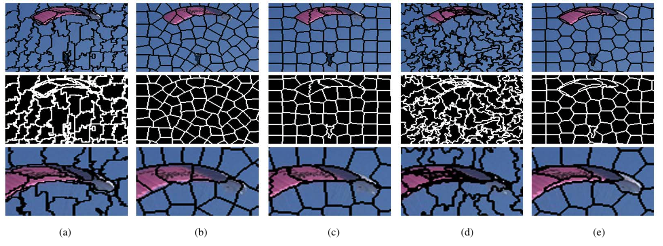
\includegraphics[width = 1 \linewidth]{images/paper2/superpixelsComparison.png}
    \centering
    \caption{Superpixel results from different algorithms. (a) SEEDS. (b) NCuts. (c) SLIC. (d) ERS. (e) LSC.}
    \label{fig: superpixelsComparison}
\end{figure}

\subsection{APPLICATIONS}
\subsubsection{Class Segmentation}
An SVM-based multi-class object classifier trained on the histograms of the generated 
superpixels was used. In order for similar superpixels to have the same 
label, a conditional random field (CRF) is used to refine the segmentation. 
Thanks to this model, the prediction made by the classifier will also 
take into account the neighbors superpixels to the one to be labeled. The 
method used is that proposed in \cite{0781426534} where the main unit of measurement is 
that of the superpixel. In \cite{0781426534} the quick shift (\emph{QS}) algorithm is used for the 
generation of superpixels. The experiments were conducted on the \emph{Graz-02} 
database \cite{0781426535} containing already labeled objects. The accuracy achieved by 
the QS, ERS, SLIC and LSC algorithms is that shown in the Table \ref{table accuracy}, while 
the various segmentations, obtained from each of these, are visible in the 
figure \ref{fig: superpixelSegmentation}. As you can see, LSC performs a better segmentation than the other 
methods, this happens because the information obtained from the histograms 
belonging to the SIFT of different superpixel generated are used. In this way 
there is a better adherence to the boundary of each object in addition the 
superpixels take on a highly irregular shape for objects in the foreground and 
more regular for the background.
\begin{table}[h!]
    \centering
    \begin{adjustbox}{max width=\textwidth}
    \begin{tabular}{*{5}{|c}|}%%{|c|c|c|c|c|}
        \hline
        & QS & ERS & SLIC & LSC\\
        \hline
        bike & 72.2 & 74.2 & 76.3 & \bfseries{76.9}\\
        cars & 72.2 & 74.7 & 72.5 & \bfseries{76.8}\\
        person & 66.3 & 66.5 & 66.7 & \bfseries{67.0}\\
        \hline
    \end{tabular}
    \end{adjustbox}
    \caption{Accuracy using different superpixels algorithms.}
    \label{table accuracy}
\end{table}

\begin{figure}[htbp]
    \centering
    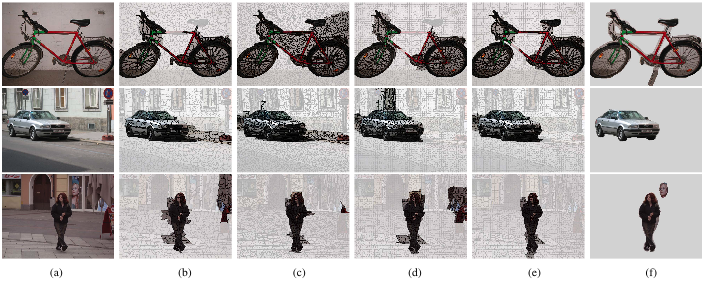
\includegraphics[width = 1 \linewidth]{images/paper2/superpixelAlgo.png}
    \centering
    \caption{Segmentation using different superpixels algorithms. (a) Original Image. (b) QS. (c) ERS. (d) SLIC. (e) LSC. (f)Ground Truth.}
    \label{fig: superpixelSegmentation}
\end{figure}

\subsubsection{Weakly Supervised Semantic Segmentation}
\begin{figure}[h!]
    \centering
    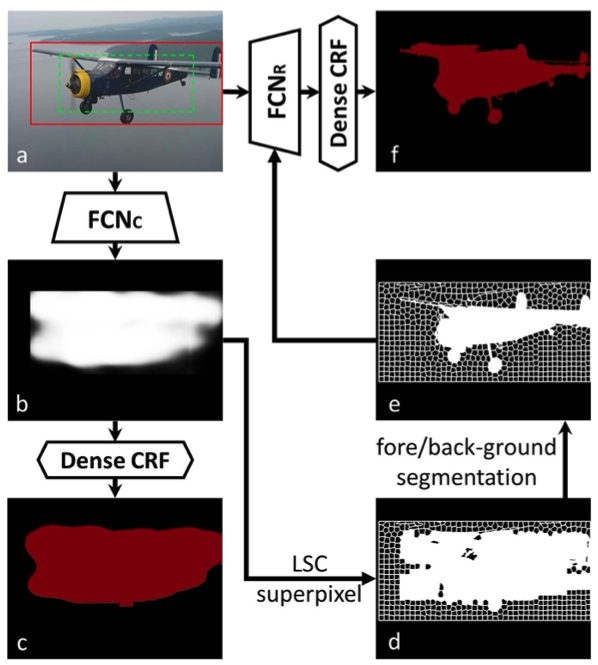
\includegraphics[width = 0.6 \linewidth]{images/paper2/semanticSegmentation.png}
    \centering
    \caption{Weakly supervised semantic segmentation. (a) A training image with bounding boxes. (b) Output of soft-max layer of $ FCN_c $. (c) Coarse semantic segmentation result. (d) Superpixels with higher probability of foreground. (e) Fore-/Background segmentation result after iterative optimization. (f) Refined semantic segmentation result.}
    \label{fig: flowchartSemanticSegmentation}
\end{figure}
As the title suggests, the LSC algorithm is able to improve semantic segmentation 
with a weakly supervised method. The images of the PASCAL 
VOC2012 database \cite{0781426538} are used as tests, in which there are 1449 images
containing labeled objects and the remaining 10582 images containing only 
bounding boxes used for training and validation. The flow chart of the proposed 
method can be seen in figure (\ref{fig: flowchartSemanticSegmentation}). The steps are as follows: coarse 
semantic segmentation, fore-/background segmentation and refined semantic 
segmentation. In the first step there is a completely convolutional network, 
called $ FCN_c $, trained with images containing only the bounding boxes which 
will be restricted in order to eliminate the border pixels that seem to be 
irrelevant. These new squares are used as positive examples, while the cut 
parts are used as negative examples. For each superpixel \emph{p} generated within 
each bounding box $ i_{th} $, we set $ c_p^i $ as the average value of the colors of each 
pixel within the superpixel and then we set $ l_p^i $ as the label to be estimated (0 
backgroud, 1 foreground). The separation of the background from the 
foreground is seen as an optimization problem
\begin{equation}
    \begin{split}
        \argmax\limits_{l} \sum_i\sum_p(E_a(l_p^i,c_p^i) + \lambda_1E_c(l_p^i, FCN_c)\\
        + \lambda_2\sum_{q\in N(p)}E_s(l_p^i,c_p^i,l_q^i,c_q^i)) 
    \end{split}
\end{equation}
Where $ E_s $ is useful for capturing the smoothness prior produced by a covariance 
matrix, $ E_c $ represents the probability that the superpixel belongs 
to the foreground, while $ E_a $, also called the appearance model, represents 
the probability that a superpixel belongs to the background or foreground. 
After several iterations, which have the purpose of updating the foreground 
and background labels of the superpixels, a correct segmentation will be 
obtained. The segmentation obtained will be used to train a convolutional 
network called $ FCN_r $ which is combined with a dense CRF model useful for 
formulating the final semantic segmentation model. This system is also 
called $ Joint_{sp} $. The model is compared with other supervivided methods \cite{0781426541}, 
a strong one, called \emph{Strong}, and a weak one called \emph{Bbox-seg}, the results of 
which can be seen in figure \ref{fig: semanticSegmentation}. While the accuracy, measured with the intersection 
over-union (\emph{IOU}), achieved by the systems mentioned is visible in the 
table \ref{table accuracy semantic segmentation}.

\begin{figure}[htbp]
    \centering
    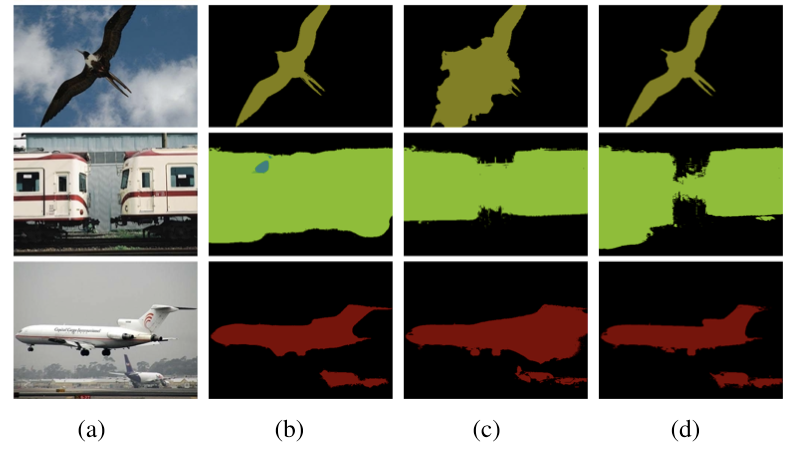
\includegraphics[width = 0.8 \linewidth]{images/paper2/segmentationAlgo.png}
    \centering
    \caption{Semantic segmentation. (a) Input image. (b) Strong. (c) Bbox-seg. (d) $ Joint_{sp} $ (LSC) }
    \label{fig: semanticSegmentation}
\end{figure}

\begin{table}[h!]
    \centering
    \begin{adjustbox}{max width=\textwidth}
    \begin{tabular}{*{3}{|c}|}%%{|c|c|c|}
        \hline
        Strong & Bbox-seg & $ Joint_{sp} $ \\
        \hline
        62.5 & 60.6 & \bfseries{64.0} \\
        \hline
    \end{tabular}
    \end{adjustbox}
    \caption{Semantic segmentation accuracy in terms of Mean IOU (\%)}
    \label{table accuracy semantic segmentation}
\end{table}

\subsection{CONCLUSIONS}
Like all superpixel algorithms, there are still two problems that need to be 
solved. The first concerns the number K of superpixels to be generated. Unfortunately, 
this parameter still has to be entered manually and today there 
is no stable method that can establish a specific K number of superpixels on 
each type of image. The second, on the other hand, concerns the study of 
new similarity techniques, instead of the one already used in this article 
($ W(p,q) $), useful for improving the performance, in terms of segmentation, 
of LSC.

\newpage
\section{An End-to-End Compression Framework Based
on Convolutional Neural Networks}

\begin{flushleft}
    \author{
    Feng Jiang, 
    Wen Tao, 
    Shaohui Liu, 
    Jie Ren, 
    Xun Guo, 
    Debin Zhao, 
    \emph{Member, IEEE}
    }
\end{flushleft}

\begin{center}
    \emph{IEEE TRANSACTIONS ON CIRCUIT AND SYSTEMS FOR VIDEO THECNOLOGY, VOL. 28, NO. 11, OCTOBER 2018}
\end{center}

\subsection{INTRODUCTION}
In recent years, within the field of computer vision, remarkable results have 
been achieved with regard to image compression. The purpose of compression 
is to be able to transmit, or save, the entire image at low bit rates. As far as 
decompression is concerned, deblocking and denoising techniques have been 
developed that are useful for obtaining good images. Further pre-processing 
steps have been found to negatively impact in system performance. Therefore 
the proposed method uses a framework composed of two convolutional 
networks (\emph{CNNs}). The first network, called compact convolutional neural 
newtork (\emph{comCNN}), is used for compression and uses the JPEG, JPEG2000 
and BPG encoding codecs. The second network, called reconstruction convolutional 
neural network (\emph{RecCNN}), is used for image decompression. A 
first example of the work carried out by the proposed framework is visible in 
the Fig. \ref{fig:output}.
\begin{figure}[h!]
    \centering
    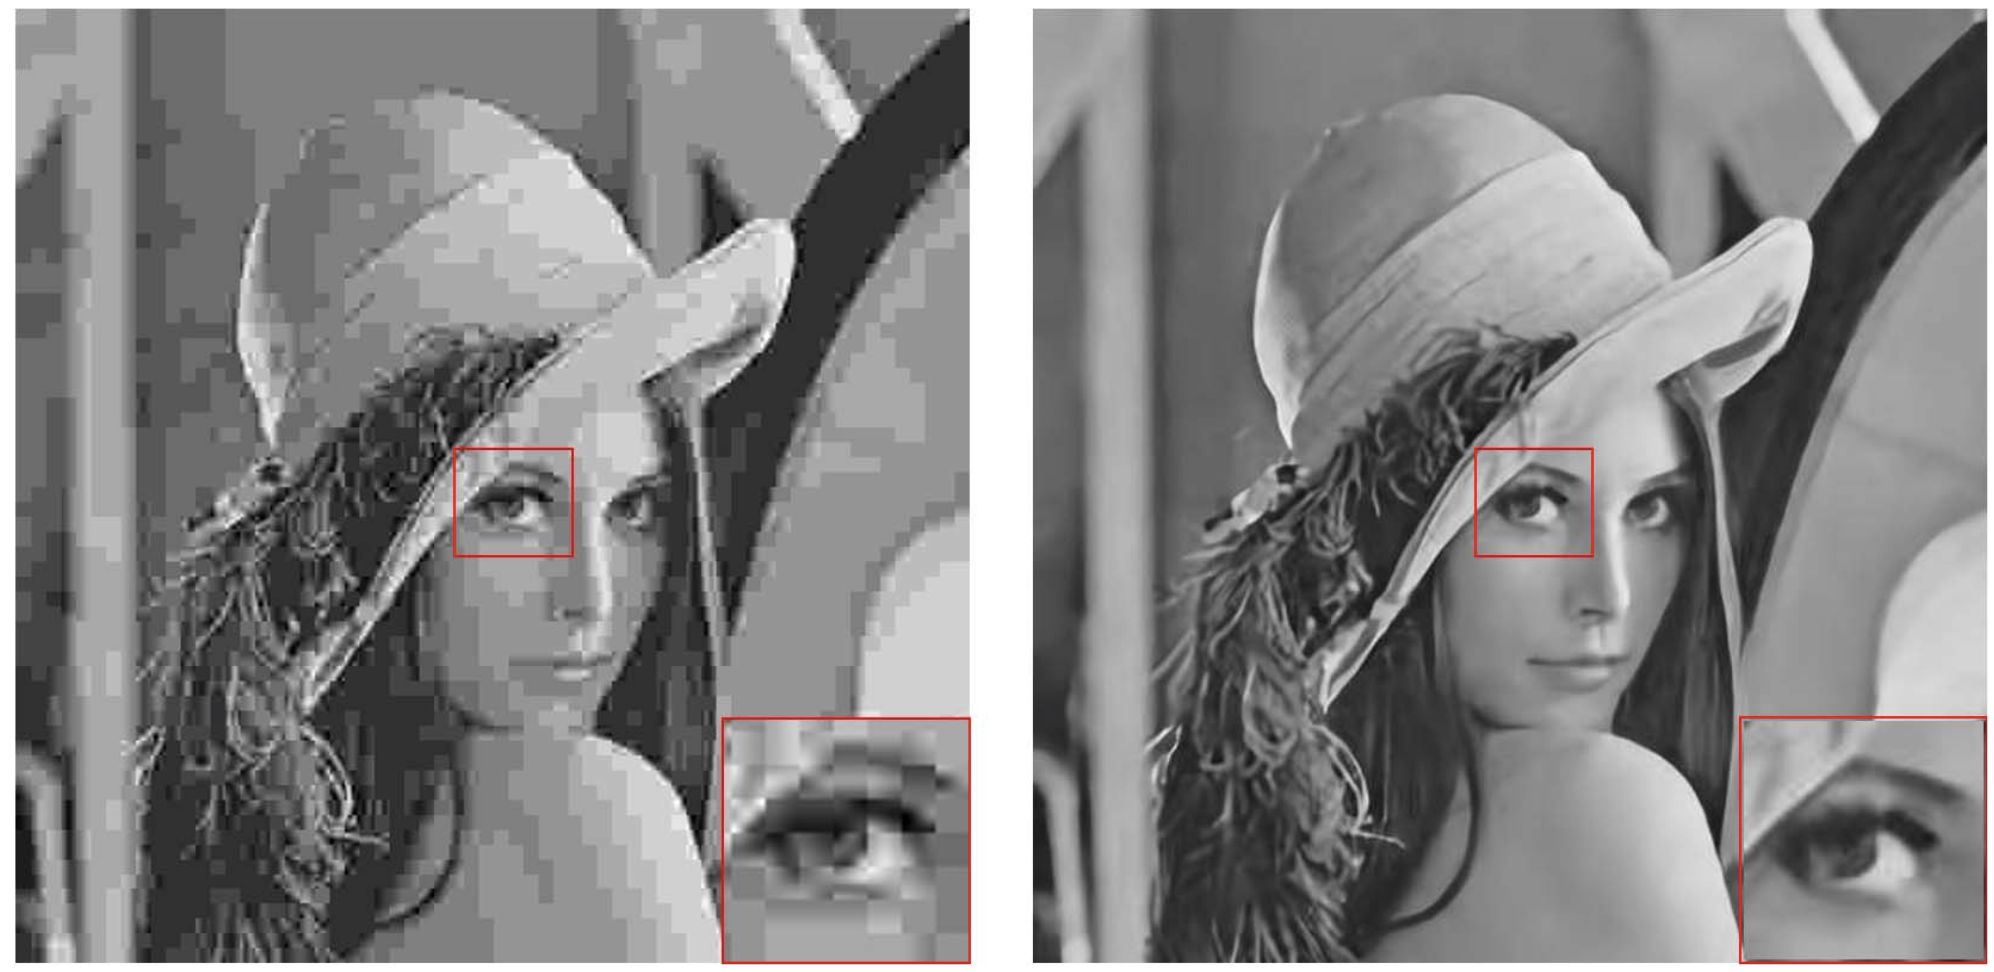
\includegraphics[width = 0.6 \linewidth]{images/paper3/output .png}
    \centering
    \caption{Left: the JPEG-coded image. Right: the decoded image.}
    \label{fig:output}
\end{figure}

\subsection{RELATED WORK}
\subsubsection{Image Deblocking and Artifacts Reduction}
Going back to talking about the deblocking technique, this is useful for removing 
all those blocks that visually worsen the appearance of each image. 
The various restoration techniques model the distortion created in the compression 
phase in order to reduce artifacts. Many methods already proposed 
in the state of the art use techniques that have a great impact on performance 
when they adopt iterative restoration processes. Therefore, the proposed 
method tries to obtain the same result but with a lower computational 
cost.

\subsubsection{Image Super-Resolution Based on Deep Learning}
Convolutional neural networks (\emph{CNNs}) have been used for super resolution 
(\emph{SR}) images especially when residual learning and gradient-based optimization 
algorithms have been proposed to train a deep network. According to 
some studies, the depth of a network doesn't always lead to good performance. 
Other researchers, on the other hand, claim the opposite.

\subsubsection{Image Compression Based on Deep Learning}
Deep learning was used for lossy and loseless compressions achieving good 
performance. There have been some methods that have prevailed over others. 
However, all of these methods ignore compatibility with various image codecs, 
thus limiting their use in some existing systems. The proposed framework 
solves this problem by operating with different image codecs, also taking into 
account the compression performance.

\subsection{THE PROPOSED COMPRESSION FRAMEWORK}
\subsubsection{Architecture of End-to-End Compression Framework}
\begin{figure}[htbp]
    \centering
    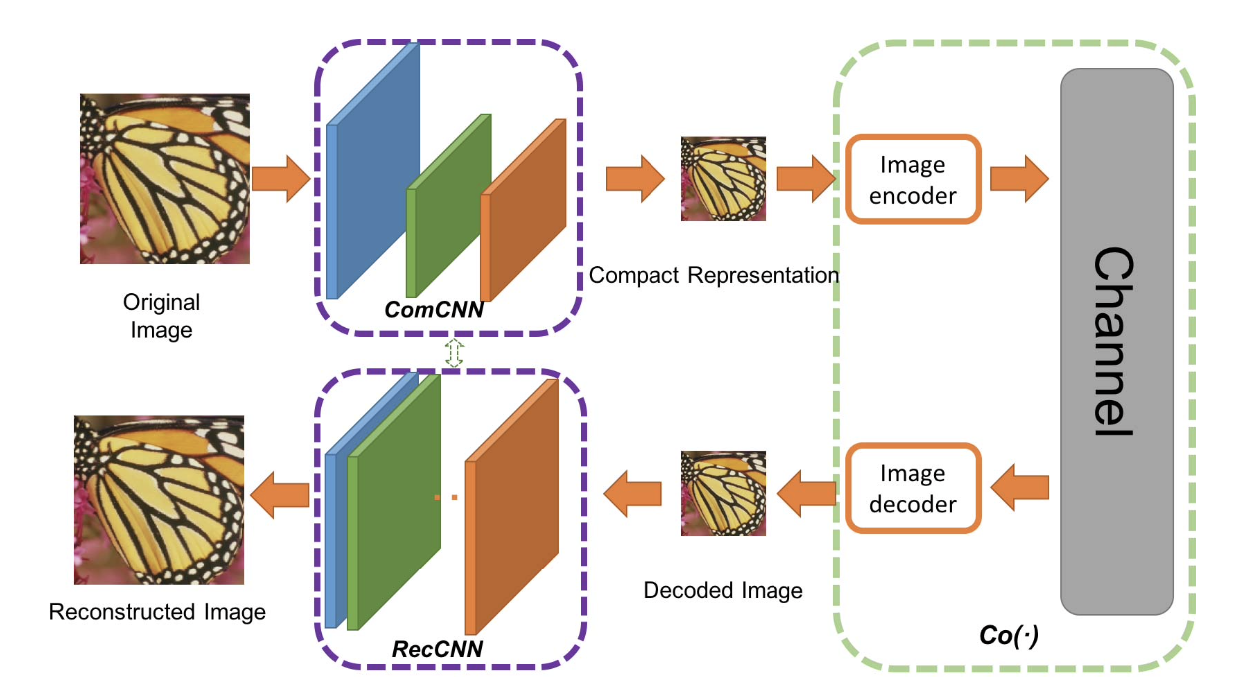
\includegraphics[width = 0.8 \linewidth]{images/paper3/framework.png}
    \centering
    \caption{The proposed novel compression framework.}
    \label{fig:framework}
\end{figure}
As mentioned, the first \emph{ComCNN} convolutional network is used to generate 
a compact representation of the input image which preserves the structural 
information and facilitates the reconstruction of image in high quality. The 
second convolutional network, \emph{RecCNN}, is used to improve the quality of the 
decoded image. In particular:
\begin{enumerate}
    \item \emph{Compact Representation Convolutional Neural Network (ComCNN)}: 
    This network is made up of three weighted layers. The first layer is 
    used to perform the extraction and representation of patches from the 
    input image. 64 filters are used, each 3x3xc in size where c indicates 
    the number of image channels. Thanks to these filters, 64 feature maps 
    are generated. The second layer has the task of downscaling and improving 
    the features with convolutional operations having stride equal to 2 
    and 64 filters of 3x3x64 size. In the last layer, \emph{c} filters, of 3x3x64 
    size, are used to reconstruct the compact representation.
    \item \emph{Reconstruction Convolutional Neural Network (RecCNN)}: The layers 
    are identical to those of the \emph{ComCNN} network, unlike the number. To 
    speed up training, as well as performance, methods such as residual 
    learning and batch normalization \cite{0799924133} are used. Finally, the image will 
    be upsampled to its original size, using a cubic interpolation.
\end{enumerate}

\subsubsection{Learning Algotrithm}
In order for both networks to have good training, their parameters must be 
optimized (weights and bias). To achieve this, the following formulas will 
have to be optimized iteratively:
\begin{equation}
    \hat{\theta_1} = \argmin\limits_{\theta_1}||Re(\hat{\theta_2},Cr(\theta_1,x))-x||^2
\end{equation}
\begin{equation}
    \hat{\theta_2} = \argmin\limits_{\theta_2}||Re(\hat{\theta_2},\hat{x}_m)-x||^2
\end{equation}
Where:
\begin{itemize}
    \item \emph{x} represents the original image
    \item $ \hat{\theta_1} $ and $ \hat{\theta_2} $ are the parameters of \emph{ComcCNN} and \emph{RecCNN}
    \item $ C_r(\cdot) $ and $ R_e() $ represent the \emph{ComcCNN} and \emph{RecCNN}
    \item $ \hat{x}_m $ is th e decoded compact representation of \emph{x}
\end{itemize}

\subsubsection{Loss Functions}
For ComCNN training: as a loss function, we use the mean square error (\emph{MSE}):
\begin{equation}
    L_1(\theta_1) = \frac{1}{2N}\sum_{k=1}^N||Re(\hat{\theta_2}, C_r(\theta1,x_k))-x_k||^2
\end{equation}
Where \emph{N} and $ \theta_1 $ represent the batch size and the trainable parameter.
For REcCNN training: after obtaining a set of compact $ x_m $ images from 
\emph{ComCNN} and the original \emph{x} images, we also use the mean square error 
(\emph{MSE}) here:
\begin{equation}
    L_2(\theta_2) = \frac{1}{2N}\sum_{k=1}^N||res(Co(\hat{x}_{mk}), \theta_2) - (Co(\hat{x}_{mk})-x_k)||^2
\end{equation}
Where $ \theta_2 $ are the trained parameters of the network while $ res(\cdot) $ represent 
the residual learning of the \emph{RecCNN}.

\subsection{EXPERIMENTS}
In order to evaluate the performance of the proposed framework, the results 
obtained were compared with six deblocking methods and two denoising 
methods. In order to train the network, the \emph{MatConvNet} \cite{0799924138} package is 
used.

\subsubsection{Datasets for Training and Testing}
For training, 400 images of 180x180 size are used. The patches used are in 
total 204800 $ (400x8x64)^2 $, with stride equal to 20. For the test, however only 
7 images are used which obviously are not present in the training ones.

\subsubsection{Model Initialization}
The initialization of the weights takes place following the method in \cite{0799924140}, 
while for the optimization of the gradient the method defined in \cite{0799924121} is used.
The training of the ComCNN network takes place in 50 epochs with a batch 
size of 128. The learning rate falls from 0.01 to 0.0001. The initial parameters 
of the second RecCNN network are identical to those of the first network, 
including the batch size.




\newpage
\section{A Data Set for Camera-Independent Color Constancy}

\begin{flushleft}
    \author{
    Ça$ \breve{g} $lar Aytekin, 
    Jarno Nikkanen, 
    Moncef Gabbouj
    \emph{Fellow, IEEE}
    }
\end{flushleft}

\begin{center}
    \emph{IEEE TRANSACTIONS ON IMAGE PROCESSING, VOL. 27, NO. 2, FEBRUARY 2018}
\end{center}

\subsection{INTRODUCTION}
Color constancy is a characteristic of the human visual system (HVS) that 
helps to perceive a constant color, for example of an object, at different levels 
of illuminations. It is claimed that the achievement of constancy occurs by 
approximating the composition of the lighting in order to obtain the true 
color of the object. There are supervised and unsupervised methods 
that calculate color consistency. Unsupervised methods are divided into two 
categories, based on the techniques they use to estimate the color of 
the illuminating source. The first category makes statistical assumptions 
about reflectance in a scene. The second category instead uses the physical 
properties of objects in scenes. Supervised methods also fall into two categories. 
The first category tries to learn a combination of unsupervised methods to 
estimate the illumination. The second category builds its own model for 
learning about illumination. The major factor affecting all of these methods 
is the sensitivity of the camera sensor. When the sets used for training, 
validation and testing contain images taken by different cameras, the results 
returned by the algorithms may be different, as well as their performance. 
On the other hand, one method returns "fixed" results when operating on 
images from the same camera. In the CC field, this problem is called camera-independence.
This report provides a dataset, called \emph{Intel-TUT}, which is 
useful for testing camera-independence in the CC. Three different cameras 
capture real scenes both in the lab and elsewhere. Laboratory images have 
different lighting conditions. The dataset contains 1536 images and a test 
set consisting of 454 images taken by a single camera.

\subsection{COLOR CONSTANCY DATASETS}
One of the first datasets for calculating the CC was the one proposed in 
\cite{0807099130}. The single camera captured images showing a total of 1995 surfaces, 
11 lab illuminations and 81 illuminations from the real world. The dataset 
also contains a number of images that make up 50 scenes. After a correct 
calibration, it removes the irrelevant images, the remainder was made up of 
only 529 images which made up 30 scenes. Each of these images belongs to 
the set captured in the lab. Another dataset is the one proposed in \cite{0807099132}, consisting 
of 11,000 images of indoor / outdoor scenes. The scenes were captured in 
different geographic locations and under different weather conditions. Unfortunately 
this dataset contains low resolution images that require a correction 
phase. Another dataset containing 246 indoor images and 322 outdoor images, 
taken by two different cameras, is the one proposed in \cite{0807099120}. Another 
dataset that uses the auto-bracketing technique to acquire the images is the 
one proposed in \cite{0807099134}. In this dataset they are acquired up to 9 different 
images, of the same scene, with different settings for each shot. A dataset that 
aims to obtain multiple lighting in a scene is the one proposed in \cite{0807099135}. 
This contains relatively few images, 9 acquired in an outdoor environment 
and 59 lab images. The is also a dataset containing the videos mentioned 
in \cite{0807099136}. There was only one study \cite{0807099129} that relies on color conversion in order 
to achieve camera independence. However, this method requires a very 
sensitive spectral camera to achieve good performance, so it is not applicable 
to all images. Finally, a last dataset consisting of 1600 indoor and outdoor 
images, taken by 9 different cameras, is the one proposed in \cite{0807099128} called NUS. 
In this collection, each scene was captured by each camera with slight misalignments. 
The database proposed in this paper is similar to the NUT only 
for the different cameras used. However, the proposed database has some 
features such as the following:
\begin{itemize}
    \item Provides the spectral sensitivities of the cameras;
    \item Different illuminants illuminate the scene;
    \item Among the different cameras used, one is mobile;
    \item Provides a set of tests for good evaluation of CC methods.
\end{itemize}

\subsection{THE PROPOSED INTEL-TUT DATA SET}
The purpose of the dataset is to help the algorithms to determine if the color 
constancy value obtained is to be considered good or not. If an algorithm 
does not find a change in this value on the same set of images taken by the 
same camera, then this algorithm is able to have a uniform color constancy 
and consequently would produce optimal outputs. Each image in the 
dataset has undergone several changes such as: black level correction (BLC), 
color shading correction (CSC) (only for mobile camera), white balance (WB), 
color conversion from RGB sensor to sRGB (CCM) , gamma correction of 
0.45, sharpening effect correction (blur) and brightness normalization.

\subsubsection{Light Sources}
A variety of devices were used that were capable of producing a light source. 
Each property such as luminance (Lux), color temperature (CCT) and CIE 
xy chromaticity, have been appropriately set to have an equitable acquisition.

\subsubsection{Cameras}
Three types of camera are used for the construction of the dataset. Two 
of these belong to the high-end, while a third belongs to the category of 
mobile. To achieve correct color correction, several 3x3 size color 
conversion matrices (\emph{CCMs}) were used. In other words, try to transform 
the components of the image from RGB to sRGB in order to adapt them to 
the lighting under which the image is viewed. For the outdoors, 10 CCMs 
were used based on the type of illumination. Another factor that required 
correction was the color shading (\emph{CS}). This only requires correction for the 
images coming from the mobile.

\subsubsection{Scene Contents}
The scenes that make up the dataset are divided into lab scenes and field 
scenes. There are several types of different lab scenes, each having 5 different 
illuminations (Fig. \ref{fig:Lab}). Both the lab scenes and those acquired in the field 
are 64, for a total of 128 scenes. Each lab scene is captured with each camera 
in almost the same shot. An attempt was made to preserve the same settings 
in the field scenes even if the latter have different lighting. In order to have 
good stabilization, a fixed tripod is used.
\begin{figure}[htbp]
    \centering
    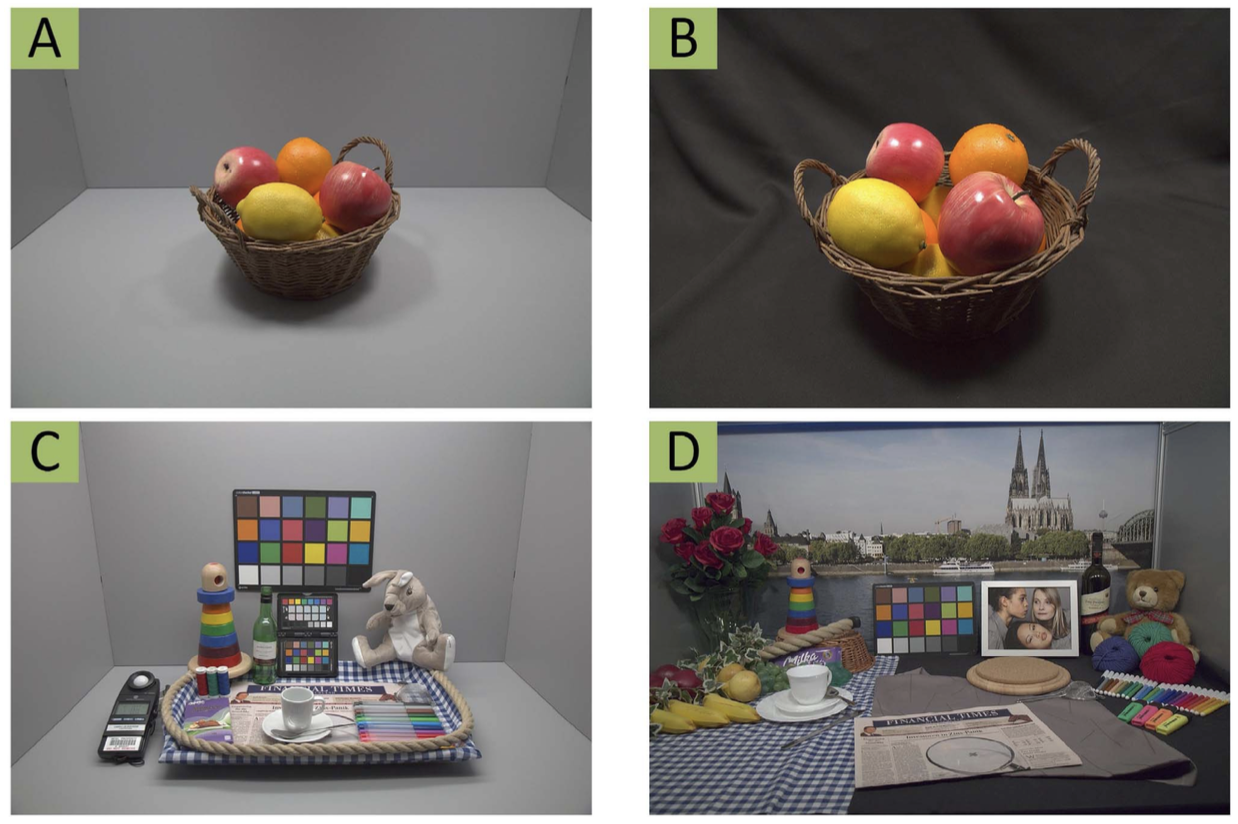
\includegraphics[width = 0.6 \linewidth]{images/paper4/lab.png}
    \centering
    \caption{Lab real scenes}
    \label{fig:Lab}
\end{figure}

\subsubsection{Ground Truths}
The ground-truth is based on the chromaticity of the illumination, or white 
points, assumed by the camera which can change for each image. This parameter 
is calculated by averaging the achromatic colors present in the lighter 
patches of the color-checker, that appear in the last line.

\subsubsection{Recommendations for Evaluating CC Algorithm Performance}\label{recommend}
In order to evaluate the performance of the algorithm with this type of 
dataset, it is recommended to use the following strategies:
\begin{enumerate}
    \item \emph{Camera independence}: the article proposes six-fold cross validation, 
    where each fold, divided into training, validation and test, contains a 
    grouping of images for each of the nine cameras. This technique aims 
    to obtain a fair evaluation of camera-independence of an algorithm (the 
    algorithm considers all images as if coming from the same camera).
    \item \emph{Camera and Scene Independence}: in this case it is recommended to 
    use the images acquired by Nikon and the mobile for training, while 
    the Canon images must be used for validation. As for the test, it is 
    recommended to use the Canon images belonging to the second group 
    of images. In this way you can understand the influence of camera-
    independence. If you get a low error, which means that the algorithm 
    treats each scene (each made up of images captured by different cameras) 
    as if it had been captured entirely by a single camera, then at 
    this point you would get, in addition to independence of the camera, 
    the independence of the scene. This is a good result if it is achieved in 
    this type of dataset.
    \item \emph{Camera and Scene Independence from Single Camera}: in this strategy 
    it is suggested to use the images from the second group as training 
    and validation while using the images acquired by Nikon and the 
    mobile for testing. In this way we want to understand if the algorithm 
    obtains the camera/scene independence effect with images produced 
    by another different camera (Canon). If this technique were 
    used with the 1 (where a low error implies the achievement of the 
    camera-independence) then when new images of different origin would 
    be inserted, the error would be higher than that obtained in 1, this is 
    because the camera-independence it faces the old set of cameras and not 
    the new one. It is being said that thanks to the combination of these, 
    it is possible to have a targeted camera-independence and a targeted 
    scene-independence for each new camera.
    \item \emph{Testing the Effect of Color Shading}: if you were to use the images 
    of your mobile, to test their color shading correction (CS), you could 
    enclose them all in a test set. Images that cause a high error will be 
    those that have not undergone the correction process.
    \item \emph{Testing the Effect of Resolution}: color constancy can be easily calculated 
    when the images are at high resolution. As you can guess, this 
    result is not achievable with images from a mobile phone. For this 
    reason, the dataset contains a portion of image downscaling (1080p) 
    useful for observing how the resolution can affect the performance of 
    the algorithm.
\end{enumerate}

\subsection{EXPERIMENTAL RESULTS}
\subsubsection{Evaluation of Unsupervised Baseline Methods}
In summary, in order to have the effect of the camera-independecy on a 
set of images from different cameras, it is enough to be able to calculate 
the constancy of the color which, in other words, means having to detect the 
chromaticity of the illuminate that precisely illuminates the scene. Given the 
chromaticity estimated by the algorithm ($ p^{Est} $) and the effective chromaticity 
(white point or ground truth) ($ p^E $), the performance of an algorithm can be 
evaluated based on the result returned by the recovery angular error (RAE):
\begin{equation}
    RAE=\cos^{-1}\left(\frac{p^Ep^{Est}}{||p^E||~||p^{Est}||}\right)
\end{equation}
This error index is calculated both on the performances obtained in high 
resolution images and in those obtained at low resolution. To make some 
comparison, an algorithm that has a low RAE is the unsupervised algorithm 
GW \cite{0807099104} which assumes that the average chromaticity in an image is gray. 
Even the MaxRGB algorithm \cite{0807099103} manages to have good performance 
in images where there are saturated areas where, thanks to these, the white 
point can be easily recovered. MaxRGB is currently the only algorithm that 
manages to have a low RAE even with low quality images (1080p). The 
performances of these algorithms, together with two others (SoG and GE), 
are compared in figure \ref{fig:RAE} where for each set of images (Lab 
Printouts, Lab Real Scenes, $ 1^{st} $ Field Set and $ 2^{nd} $ Field set), taken from different cameras, 
are calculated mean, median and maximum of RAE values reached for each 
image. Subsequently, in figure \ref{fig:RAEstandard} the mean, median and maximum of the 
standard deviation obtained from each image, from each algorithm, are calculated 
again. As you can see, the GW algorithm is the only one to have the 
camera-independence for all the rooms used.

\begin{figure}[htbp]
    \centering
    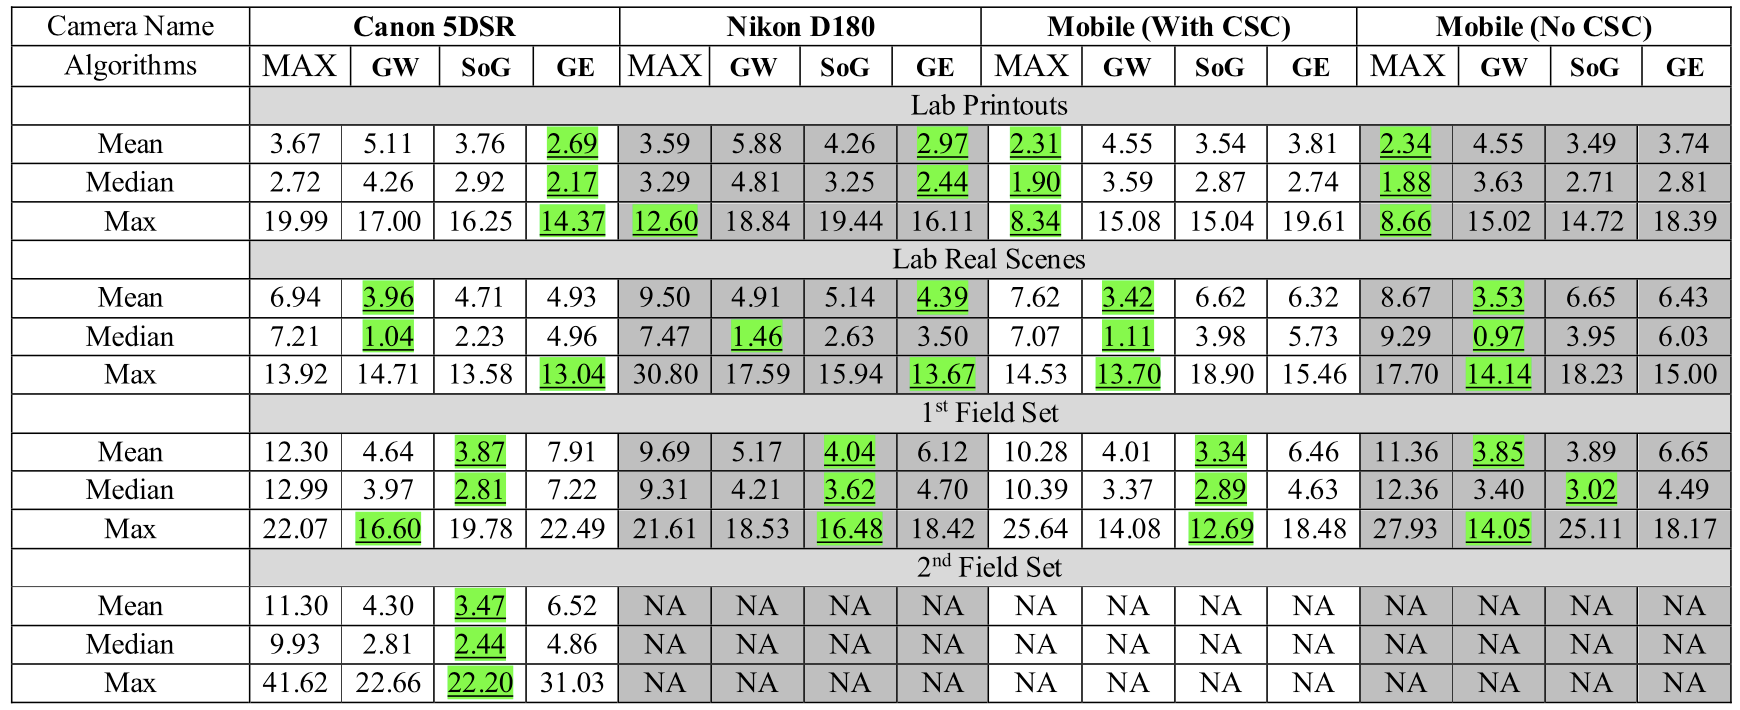
\includegraphics[width = 1 \linewidth]{images/paper4/RAEHigh.png}
    \centering
    \caption{Recovery Angular Errors (Mean, Median and Maximum) of some algorithms.}
    \label{fig:RAE}
\end{figure}

\begin{figure}[htbp]
    \centering
    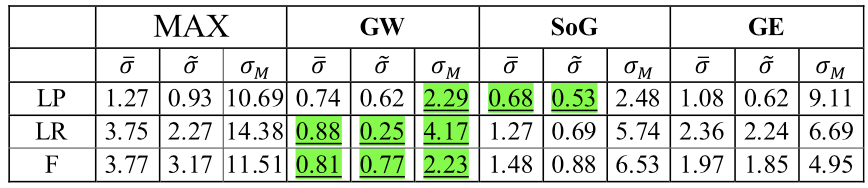
\includegraphics[width = 0.6 \linewidth]{images/paper4/standardHigh.png}
    \centering
    \caption{Mean, Median and Maximum RAE of some algorithms.}
    \label{fig:RAEstandard}
\end{figure}

\subsubsection{Evaluation of a Direct Supervised Method}
In order to be able to calculate color constancy, and thus be able to achieve 
the camera-independence, various methods were used that included the use 
of convolutional neural networks (CNNs). In method \cite{0807099122}, the network used 
is composed of a convolutional layer with 240 filters of size 1x1, the usual 
function of ReLU, a max-Pooling of blocks of size 8x8 with stride 8. Finally 
there is a fully-connected layer with 40 layers hidden and a 3-dimensional 
output in which there is the estimated chromaticity of the lighting. In order to demonstrate the validity of the proposed dataset, the use of CNN has been adapted to the techniques described in \ref{recommend}:
\begin{enumerate}
    \item Following technique 1, various CNNs are trained to provide the least 
    possible error. The error reached by the model is less than when using 
    the Canon for training and validation. This means that the networks 
    assume the camera-independence only with the Nikon and mobile models. 
    Therefore the networks would be able to recognize new cameras. As 
    can be seen in the figure, the RAE values between the various cameras 
    are very similar (Fig. \ref{fig:CNNtec1}).
    \begin{figure}[htbp]
        \centering
        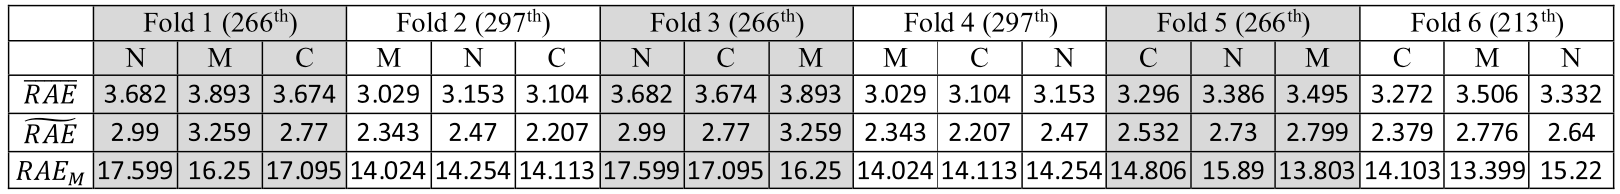
\includegraphics[width = 1 \linewidth]{images/paper4/CNNtec1.png}
        \centering
        \caption{Camera Independence of \cite{0807099122} with CCM on $ 1^{rst} $ thecnique. Mean, Median and Maximum RAE of CNN.}
        \label{fig:CNNtec1}
    \end{figure}
    \item Now a CNN is trained using technique 2. The training is carried out 
    with images acquired from both Nikon and mobile. Canon's images are 
    used for validation, while Canon's images belonging to the $ 2^{nd} $ field 
    are used for the test. Low errors are obtained with the use of a color 
    conversion matrix (CCM) \cite{0807099129} and therefore the model manages to have 
    the camera/scene-independence (Fig. \ref{fig:CNNtec2}).
    \begin{figure}[h!]
        \centering
        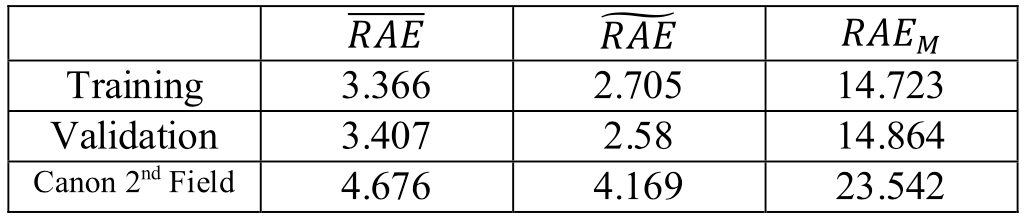
\includegraphics[width = 0.6 \linewidth]{images/paper4/CNNtec2.png}
        \centering
        \caption{Camera Independence of \cite{0807099122} with CCM on $ 2^{nd} $ thecnique. Mean, Median and Maximum RAE of CNN.}
        \label{fig:CNNtec2}
    \end{figure}
    \item According to technique 3, a CNN can be trained to reach camera independence 
    only on one camera, excluding the others. In this case, since 
    the images of the $ 2^{nd} $ field, used for both training and validation, belong 
    only to Canon, then CNN will get the camera/scene-independence 
    only on this type of camera (Fig. \ref{fig:CNNtec3}).
    \begin{figure}[h!]
        \centering
        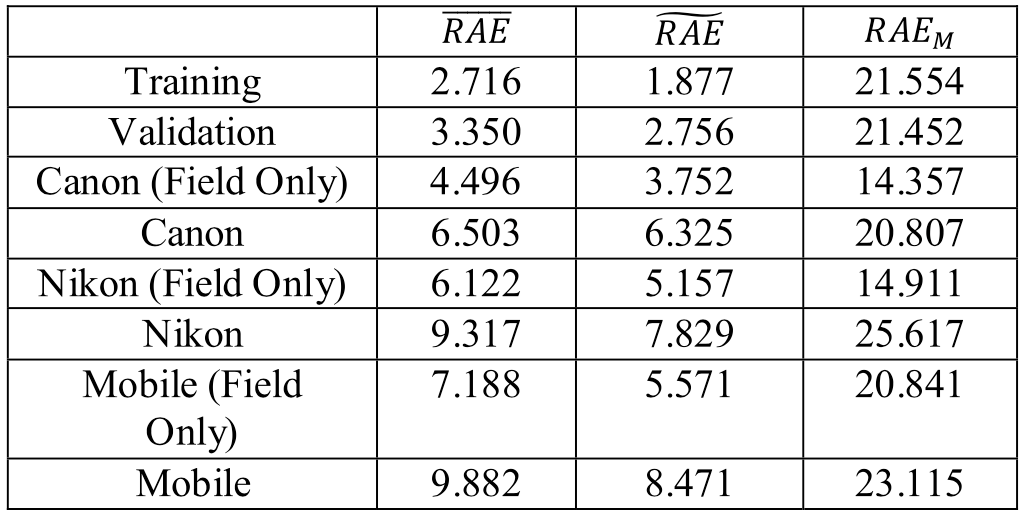
\includegraphics[width = 0.6 \linewidth]{images/paper4/CNNtec3.png}
        \centering
        \caption{Camera Independence of \cite{0807099122} on $ 3^{nd} $ thecnique. Mean, Median and Maximum RAE of CNN.}
        \label{fig:CNNtec3}
    \end{figure}
\end{enumerate}

\subsubsection{A State of the Art Camera Independent Method}
The following section presents a competitive method \cite{0807099125} that can beat the 
performance of \cite{0807099122}. Also in this new method there is an even deeper CNN 
that uses a set of images on which a CCM pre-processing phase has already 
been applied. The comparisons of the results obtained by \cite{0807099122} and by \cite{0807099125} in 
all the techniques proposed in \ref{recommend} where it can be seen that all the error 
rates of \cite{0807099125} are smaller than those of \cite{0807099122} and therefore the model is able to 
reach the camera/scene-independece more easily.
\begin{figure}[htbp]
    \centering
    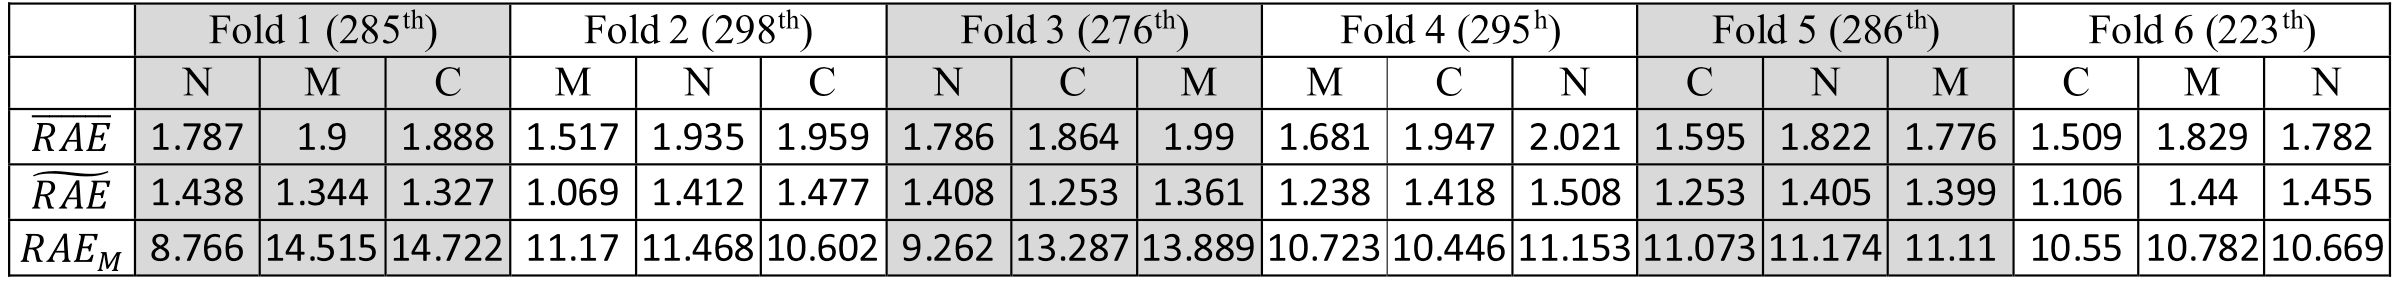
\includegraphics[width = 1 \linewidth]{images/paper4/25tech1.png}
    \centering
    \caption{Camera Independence of \cite{0807099122} with CCM on $ 1^{nd} $ thecnique. Mean, Median and Maximum RAE of CNN.}
    \label{fig:25t1}
    \begin{minipage}[t]{.45\linewidth}
        \centering
        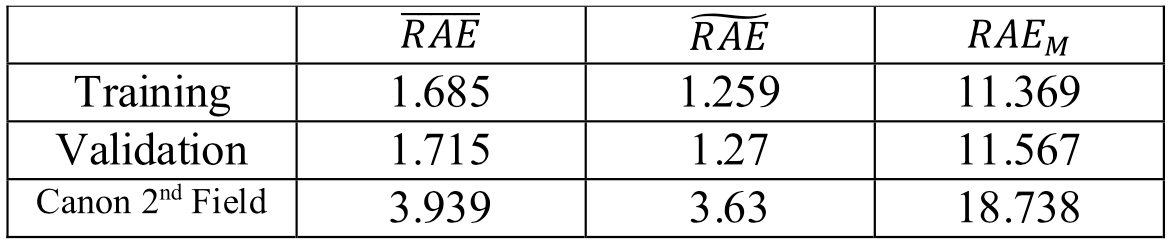
\includegraphics[width=\linewidth]{images/paper4/25tech2.png}
        \caption{\small Camera Independence of \cite{0807099122} on $ 2^{nd} $ thecnique. Mean, Median and Maximum RAE of CNN.}\label{fig:1}
    \end{minipage}
    \hfill
    \begin{minipage}{.45\linewidth}
        \centering
        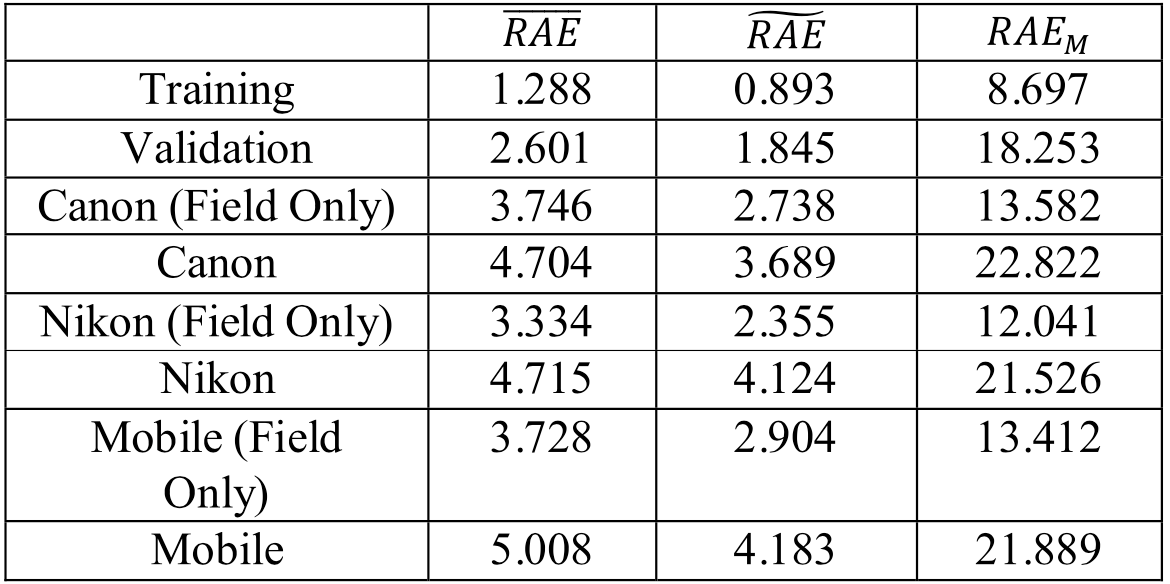
\includegraphics[width=\linewidth]{images/paper4/25tech3.png}
        \caption{\small Camera Independence of \cite{0807099122} on $ 3^{nd} $ thecnique. Mean, Median and Maximum RAE of CNN.}\label{fig:1}
    \end{minipage}  
    \label{fig:1-2}
\end{figure}

\subsection{CONCLUSION}
The dataset proposed in this paper is useful for testing the behavior of 
an algorithm, or a model based on CNN, in the search of camera/scene-independece. 
If the algorithm manages to obtain this benefit, then it will be 
able to generalize a scene composed of several images acquired from different 
cameras, otherwise the results returned by this will be highly variable. 
Achieving this goal can also be done using a CNN if the CMM process is 
applied to its input set. It is necessary to specify that, in order to 
achieve the final result, it is essential to have the spectral sensitivities of each camera 
without which it would not be possible to achieve camera independence.

\newpage
\section{An End-to-End Multi-Task and Fusion CNN for Inertial-Based Gait Recognition}

\begin{flushleft}
    \author{
    Rubén Delgrado-Esca$ \tilde{n} $o,
    Francisco M. Castro,
    Julián Ramos Cózar,
    Manuel J. Marín-Jiménez,
    and Nicolás Guil
    }
\end{flushleft}

\begin{center}
    \emph{IEEE DIGITAL OBJECT IDENTIFIER}
\end{center}

\subsection{INTRODUCTION}
An individual's gait appears as their own fingerprint. The study of this 
topic doesn't not only concern the area of medicine, but also that of security 
and identification. The gating study is based on a non-invasive system that 
collects patterns without the direct intervention of the subject. The data, 
which allow the recognition of the gait, are taken by inertial sensors present 
in a multitude of devices such as smartphones or smartwatches. A system 
is presented that uses a convolutional neural network (CNN) that uses the 
data collected by these inertial sensors to be able to predict the subject. The 
approach followed is the one in figure \ref{fig:preview}. Two extensions have been added 
to the network. The first deals with merging sensory data, while the second 
deals with improving the learning process and producing multiple outputs 
from a single input, thanks to a multi-task scheme. The tasks considered 
are: identification, gender recognition and age estimation. The dataset used 
is OU-ISIR gait database \cite{0857651721}, containing information such as inertial sensors 
such as accelerometers and gyroscopes.
\begin{figure}[htbp]
    \centering
    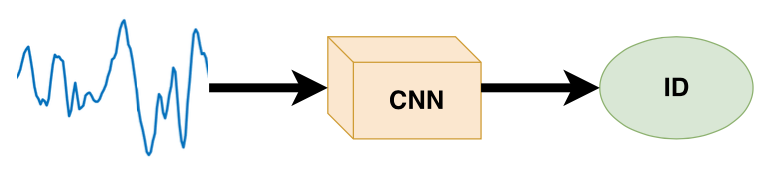
\includegraphics[width = 0.6 \linewidth]{images/paper5/usecase.png}
    \centering
    \caption{A preview of how the model works.}
    \label{fig:preview}
\end{figure}

\subsection{RELATED WORK}
Some methods have placed inertial sensors in different parts of the body 
such as legs \cite{0857651733}, hips \cite{0857651732}, ankles, or even in objects such as bags [35] and 
pockets \cite{0857651720}. Other methods \cite{0857651736} directly use all the inertial sensors present 
in the smartphone. With the advent of deep learning and CNNs, classifying 
an activity has turned out to be an easier job. The input provided to these 
networks is either the raw data of the inertial sensors, or the images that 
represented such data. The entire sequence of data is divided into segments, 
or windows, in order not to negatively affect the performance of the network. 
In the following work, a union of all the data produced by inertial sensors is 
carried out with the multi-task approach in order to provide a single model 
that uses different inputs to produce different outputs.

\subsection{PROPOSED APPROACH}
\subsubsection{Problem definition}
The proposed neural network is able to automatically extract the discriminat 
features from a gait sequence. There is no data pre-processing phase. The 
dataset used contains three labels for each fetature, indicating the age, years 
and gender of the subject, but in addition to this, any type of dataset with 
labels and sensory data would have been fine. In the following paper the 
following nomenclature will be used:
\begin{itemize}
    \item {\bfseries{\emph{S}}}: input temporal sequence of \emph{D} channel measurements taken by a sensor.
    \item {\bfseries{$ s_i $}}: sub-sequence of \emph{S} having length \emph{L}, given as input to CNN.
    \item $ y_i^t $: label of the sub-sequence $ s_i $ and taskt \emph{t}.
    \item $ g(s_i, \theta ) $: non-linear function applied to $ s_i $ with a set of parameters $ \theta $.
    \item {\bfseries{$ \hat{y_i} $}}: output of the network for a given $ s_i $ input.
\end{itemize}

\subsubsection{Initial CNN Architecture}
The length of the input is normalized before it can end up on CNN. Each 
sequence S is divided into U sub-sequences $ s_i $, where $ 1 \leq i \leq U $. However, 
a sequence is divided into windows having length L, with an overlap of 0\%, 
where each signal size defines a specific input channel. The number D of 
channels is useful for defining the 1 x N x D dimension of the filter of the 
first layer, where N indicates the dimension of the convolution. The proposed 
convolutional network is composed of 4 convolutional layers and a gradually 
increasing number of filters. After convolution there are elements such as 
ReLU, batch normalization (useful for faster learning) and max pooling. After 
the last convolutional layer, the average is chosen as a pooling operation. 
Then dropout and fully-connected layers are added with a number of outputs 
equal to the required classes. The last layer is composed of the Softmax 
normalization function which returns the probability distribution of each class. 
To train the model, only for the identification task, a cross-entropy is used 
as a loss function.
\begin{figure}[htbp]
    \centering
    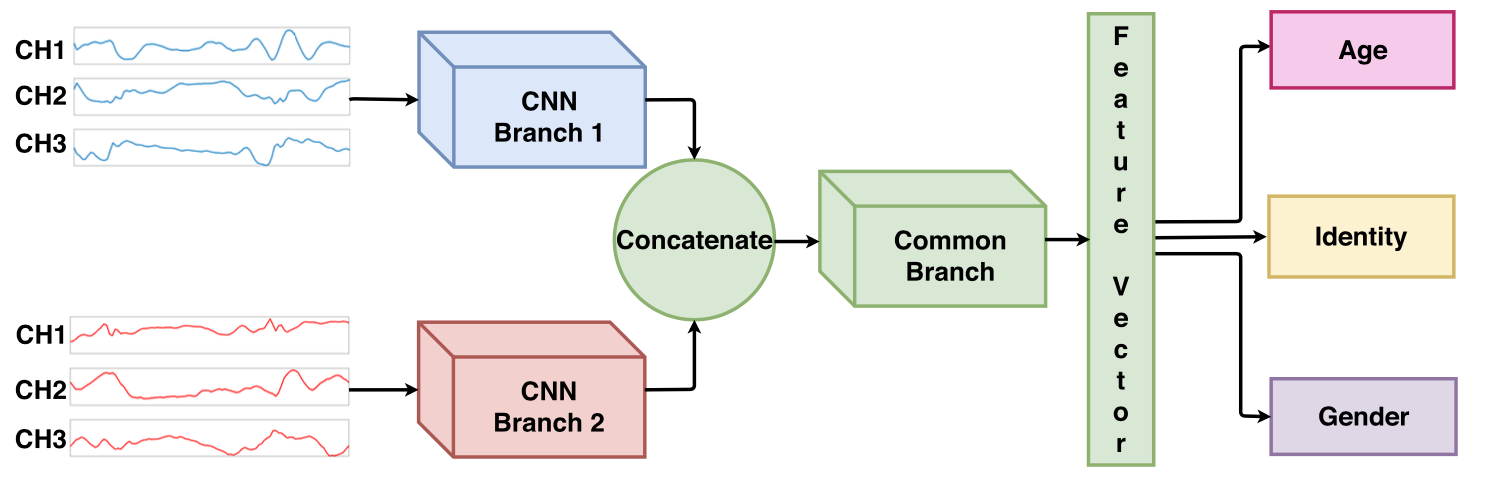
\includegraphics[width = 1 \linewidth]{images/paper5/architecture.png}
    \centering
    \caption{Pipeline for multi-task and multi-sensor learning in a gait-based system}
    \label{fig:pipeline}
\end{figure}

\subsubsection{Multi-task Approach}
The aim is to training a deep multi-task model (DTM). In order to do this, 
there must be a set of tuples $ I = (s_i, y_i^m, y_1^1, ..., y_i^T) $ where $ y_i^m $ is the label 
of the main task, $ y_i^t $, with $ t \in [1,T] $, is the label for each auxilary task. 
Each individual task has its own loss function \emph{L}. The loss function (\ref{loss-function}) is 
calculated on each sub-sequence \emph{s} and is formed by the product of each single 
loss function, of each task, with the weights ($ \lambda $)  associated at each task.
\begin{eqnarray}\label{loss-function}
    \emph{$ L_{DTM} (g(s,\theta), Y) $} & = & \lambda_{id}L_{id}(\hat{y}^{id}, y^{id}) \nonumber \\
                                        &   & + \lambda_{age}L_{age}(\hat{y}^{age}, y^{age}) \nonumber \\
                                        &   & + \lambda_{gender}L_{gender}(\hat{y}^{gender}, y^{gender}) 
\end{eqnarray}
Where $ Y = (y^{id}_i, y^{age}_i, y^{gender}_i) $ and $ L_{id}, L_{age}, L_{gender} $ are the loss functions of 
each tasks. As for the identity and gender tasks, their loss function is the 
cross-entropy and is calculated with the formula \ref{cross-entropy}.
\begin{equation}\label{cross-entropy}
    \emph{$ L_m(\hat{y}, c) $} = -\hat{y}_c+\log\sum^K_{k=1}e^{\hat{y}k} 
\end{equation}
Where $ \hat{y} $ is the ouput vector of the network, $ \hat{y}_c $ is the output for target class, 
$ \hat{y}_k $ is the \emph{k}-th component of the output vector, \emph{c} is the ground-truth class 
and \emph{K} is the total number of classes.

\subsubsection{Modality Fusion}
The merging of data that occurs at the input is useful for increasing the accuracy of the 
network and allows understanding the relationships between 
the different types of input data. Each data coming from a specific sensor 
will be inserted in an individual branch, composed of a specific number of 
convolutional layers that will calculate specific predictors for each sensor. 
In the end, the data will be concatenated in a common branch which has the 
task of extracting the combined features from all the sensors. Based on the accuracy metric, the 
layer that will return the best result will be selected.

\subsubsection{Identity Authentication}
An authentication process begins by submitting a sample of input to CNN. 
Within this, there may be a layer that will produce a vector of features. 
To find out which layer it is, a cross-validation process is performed. Once 
extracted, the features are normalized with the L2 standard. Subsequently 
a vector is calculated containing the Euclidean distances between the values 
given in input and those present in the training set. In order to calculate the 
\emph{Area Under Curve} (AUC) or the \emph{Equal-Error-Rate} (EER), these distances 
are transformed into probabilities.

\subsection{EXPERIMENTS AND RESULTS}
\subsubsection{Dataset}
The OU-ISIR dataset is composed in two parts. Part A contains data on 744 
individuals, each having two sub-sequence (s) recording at a rate of 100Hz 
via an IMU sensor located at the waist of each. The first sequence is used for 
training, the second for testing. The labels associated with each individual 
are: identity, gender and age (split in ranges). Part B, on the other hand, 
is composed of 495 individuals with 3 IMU sensors located on the body. For 
each individual and sensor, there are two sequences of walking levels, an up-slope 
walk sequence and the other down-slope walk. The data that will be 
merged are those coming from sensors such as accelerometer and gyroscope.

\subsubsection{Input data}
A data augumentation process is carried out to increase the amount of data 
available for training. In this way, instead of giving a single sequence S 
as input, three will be given, more precisely:
\begin{itemize}
    \item A Gaussian noise is added to the input signal;
    \item The sequence S is resized with a random value between 0.7 and 1.1;
    \item A sequence of 10 numbers is first interpolated to S and then the resulting sequence is sampled.
\end{itemize}
Each sequence (S) is divided into 100 sub-sequences ($ s_i $) (100Hz = 1 per 
second), a number enough to contain a walk, with overlap equal to 75\%.

\subsubsection{Implementation details}
First 100 epochs are performed in order to train the model, with the training 
set divided into training and validation. At the end of the training, in order to 
be able to fine-tune the parameters, a further 50 epochs are performed with 
the training set only. The optimization is carried out with the stochastic 
gradient descent (SGD) standard with a mini-batch of 128 samples, weigth 
decay of 0.0005 and a moment of 0.9. The total accuracy is obtained by 
combining the accuracies derived from the output of each sub-sequence ($ s_i $) 
of the input S. To obtain this, simply multiply each probability obtained 
from each of the sub-sequences with the following equation:
\begin{equation}
    P(S=c) = \prod_{i=1}^UP_i(s_i=c)
\end{equation}
Where U is the number of subsequences $ s_i $, P(s=c) is the probability of assign the identity \emph{c} to the person in sequence S and $ P_i(s_i=c) $ is the probability of assign the identity \emph{c} to teh person in subsequence $ s_i $.

\subsubsection{Gait Recognition experiments}
Different types of experiments and their respective performances, in terms of accuracy and F1-measure, are presented below.
\begin{enumerate}
    \item \emph{Sensor position}: the following experiment show that using 3 different 
    sensors, the model has greater accuracy and a high value of F1-measure, 
    when using data from the sensor positioned on the left side of the body.
    \begin{table}[h!]
        \centering
        \begin{adjustbox}{max width=\textwidth}
        \begin{tabular}{*{3}{|c}|}%%{|c|c|c|}
            \hline
            IMU Position & Acc & F1-score \\
            \hline
            center & 92.3 & 90.8\\
            left & \bfseries{95.2} & \bfseries{94.0}\\
            right & 91.5 & 90.0\\
            \hline
        \end{tabular}
        \end{adjustbox}
        \caption{Accuracy and F1-score of three different sensors.}
        \label{table accuracy and F1}
    \end{table}

    \item \emph{Single task with individuals sensors} (1 Task, 1 Sensor): being a multi-task 
    network, a CNN network is created for each sensor in combination 
    with each label. As there are three types of labels and two sensors, a 
    total of 6 CNN networks are trained. From the results obtained from 
    the experiment, it can be seen that both sensors affect the model in an 
    almost similar way, in terms of accuracy and F1-Measure. These values 
    indicate that both sensors can be used in order to achive the purpose 
    of identifying the walk.
    \begin{table}[h!]
        \centering
        \begin{adjustbox}{max width=\textwidth}
        \begin{tabular}{|c||ccc|c||ccc|c|}
            \hline
                & \multicolumn{4}{c||}{Acc} & \multicolumn{4}{c|}{F1-Score} \\
            \hline
                Architecture & Id & Age & Gender & Avg & Id & Age & Gender & Avg\\
            \hline
                SingleTask Accelerometer & 89.7 & 91.0 & 94.8 & 91.8 & 87.6 & 91.3 & 94.5 & 91.2\\
                SingleTask Gyroscope& 89.1 & 89.1 & 94.4 & 90.9 & 87.5 & 89.7 & 94.4 & 90.5\\
            \hline 
        \end{tabular}
        \end{adjustbox}
        \caption{Accuracy and F1-score (1 Task, 1 Sensor).}
        \label{table accuracy and F1 (1 Task - 1 Sensor)}
    \end{table}

    \item \emph{Multi-task with individual sensors} (+ Task, 1 Sensor): in this experiment 
    more tasks are assigned to each of the sensors (3 tasks for 1 
    sensor) implying the creation of two CNN networks. This experiment 
    is useful to see if there are any performance improvements with respect 
    to the single assignment (defined in the previous point). The loss function 
    is that described in equation \ref{loss-function}. Comparing the results obtained 
    in table \ref{table accuracy and F1 (1 Task - 1 Sensor)} with table \ref{table accuracy and F1 (more Task - 1 Sensor)}, it can be seen that the following experiment led 
    to a slight improvement in performance.
    \begin{table}[h!]
        \centering
        \begin{adjustbox}{max width=\textwidth}
        \begin{tabular}{|c||ccc|c||ccc|c|}
            \hline
                & \multicolumn{4}{c||}{Acc} & \multicolumn{4}{c|}{F1-Score} \\
            \hline
                Architecture & Id & Age & Gender & Avg & Id & Age & Gender & Avg\\
            \hline
                MultiTask Accelerometer & 90.9 & 93.3 & 95.9 & 93.4 & 89.1 & 93.3 & 95.9 & 92.8\\
                MultiTask Gyroscope & 90.1 & 90.1 & 94.8 & 91.7 & 88.3 & 90.5 & 94.9 & 91.2\\
            \hline 
        \end{tabular}
        \end{adjustbox}
        \caption{Accuracy and F1-score (+ Task, 1 Sensor).}
        \label{table accuracy and F1 (more Task - 1 Sensor)}
    \end{table}

    \item \emph{Selection of the fusion position}: The fusion can take place in any convolutional 
    layer, called the common branch, of the network. For each 
    layer, a number of filters are applied which increases as the 
    depth of the network increases. As can be seen from table \ref{table accuracy and F1 fusion}, the best performances 
    are obtained in the fusion obtained in the first convolutional layer of 
    the network. Subsequent convolutional layers score lower because the 
    amount of information used for training is low.
    \begin{table}[h!]
        \centering
        \begin{adjustbox}{max width=\textwidth}
        \begin{tabular}{*{3}{|c}|}%%{|c|c|c|}
            \hline
            Position & Acc & F1-score\\
            \hline
            Conv1 & \bfseries{94.2} & \bfseries{92.9}\\
            Conv2 & 94.0 & 92.7\\
            Conv3 & 93.4 & 92.0\\
            Conv4 & 89.0 & 86.7\\
            Conv5 & 89.0 & 86.7\\
            \hline
        \end{tabular}
        \end{adjustbox}
        \caption{Accuracy and F1-score of fusion level experiment.}
        \label{table accuracy and F1 fusion}
    \end{table}

    \item \emph{Single Task with Fusion} (1 Task, + Sensor): in this experiment 3 CNNs 
    are used, one for each task, each making up a branch. In this case, the 
    combination of data from different sensors will be useful to be able to 
    determine only 1 task and therefore only one class. The results obtained 
    are better than the previous points, except for the gender class where 
    the MultiTask approach achieves a better score.
    \begin{table}[h!]
        \centering
        \begin{adjustbox}{max width=\textwidth}
        \begin{tabular}{|c||ccc|c||ccc|c|}
            \hline
                & \multicolumn{4}{c||}{Acc} & \multicolumn{4}{c|}{F1-Score} \\
            \hline
                Architecture & Id & Age & Gender & Avg & Id & Age & Gender & Avg\\
            \hline
                SingleTask Fusion & 94.2 & 95.0 & 95.6 & 94.9 & 93.5 & 95.0 & 95.6 & 94.7\\
            \hline 
        \end{tabular}
        \end{adjustbox}
        \caption{Accuracy and F1-score (1 Task, + Sensor).}
        \label{table accuracy and F1 (1 Task, + Sensor)}
    \end{table}

    \item \emph{Multi-task with Fusion} (+ Task, + Sensor): the last experiment consists in applying the fusion in a multitasking context within the network. In this case it will be necessary to train a CNN for all three existing tasks. From the results shown in table \ref{table accuracy and F1 (+ Task, + Sensor)}, this architecture manages to achieve better performance than the others mentioned above, this is because the model has much more information (labels and inputs) to describe people. The strength of this architecture is that it manages to return a result for each task.
    \begin{table}[h!]
        \centering
        \begin{adjustbox}{max width=\textwidth}
        \begin{tabular}{|c||ccc|c||ccc|c|}
            \hline
                & \multicolumn{4}{c||}{Acc} & \multicolumn{4}{c|}{F1-Score} \\
            \hline
                Architecture & Id & Age & Gender & Avg & Id & Age & Gender & Avg\\
            \hline
                MultiTask Fusion & \bfseries{94.8} & \bfseries{96.1} & \bfseries{97.7} & \bfseries{96.2} & \bfseries{93.8} & \bfseries{96.3} & \bfseries{97.7} & \bfseries{95.9}\\
            \hline 
        \end{tabular}
        \end{adjustbox}
        \caption{Accuracy and F1-score (1 Task, + Sensor).}
        \label{table accuracy and F1 (+ Task, + Sensor)}
    \end{table}

\end{enumerate}

\newpage
\bibliographystyle{abbrv}
\bibliography{Bibliography}


\end{document}